% Titre de la deuxième partie
\section{Résolution naïve}

\begin{frame}
    \tableofcontents[currentsection]
\end{frame}

%%%%%%%%%%%%%%%%%%%%%%%%%%%%%%%%%%%%%%%%%%%%%%%%
% Première diapo
%%%%%%%%%%%%%%%%%%%%%%%%%%%%%%%%%%%%%%%%%%%%%%%%
\begin{frame}
\frametitle{Résolution naïve}
\framesubtitle{Méthode}

\begin{enumerate}
    \item<1-> Construire la carte en discrétisant les coordonnées
    \item<2-> Propager depuis les obstacles la distance de sécurité
    \item<3-> Calculer un chemin via un algo classique (A* ou Dijkstra)
\end{enumerate}

\begin{figure}
    \centering
    \visible<1->{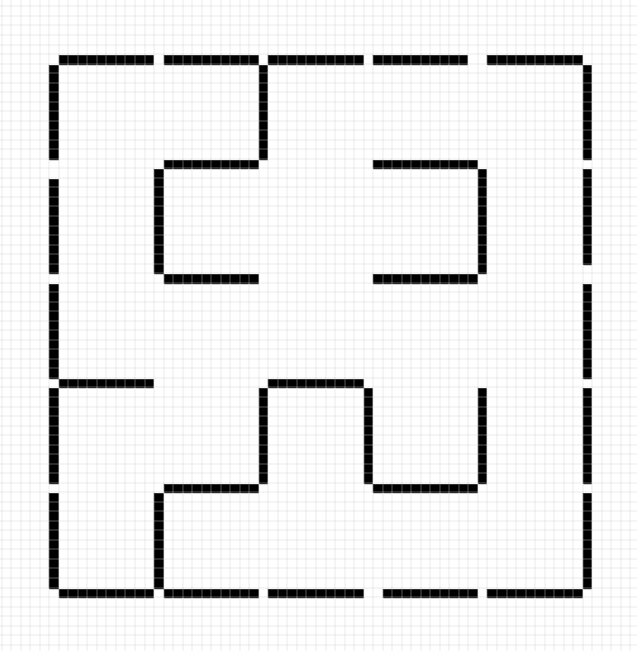
\includegraphics[width=0.4\linewidth]{assets/naif_0.png}}
    \qquad
    \visible<2->{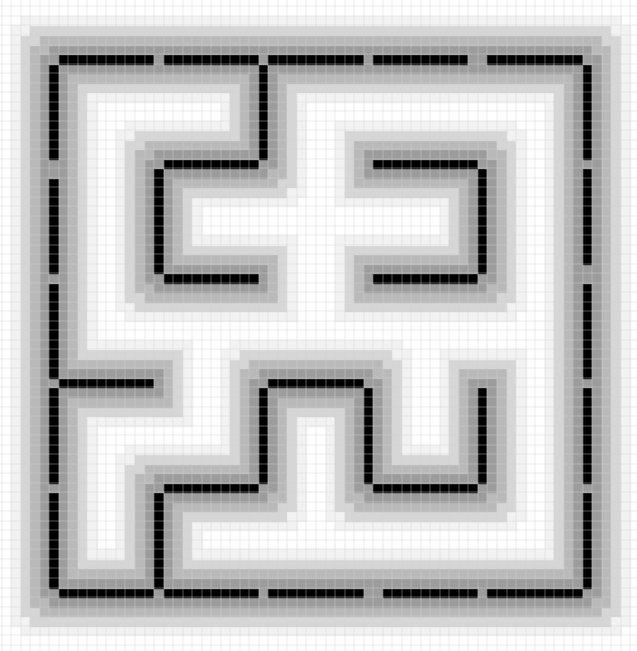
\includegraphics[width=0.4\linewidth]{assets/naif_1.png}}
\end{figure}

\end{frame}

%%%%%%%%%%%%%%%%%%%%%%%%%%%%%%%%%%%%%%%%%%%%%%%%
% Deuxième diapo
%%%%%%%%%%%%%%%%%%%%%%%%%%%%%%%%%%%%%%%%%%%%%%%%
\begin{frame}
\frametitle{Résolution naïve}
\framesubtitle{Un premier résultat !}
\begin{columns}
    \begin{column}{.55\textwidth}
        \begin{figure}
            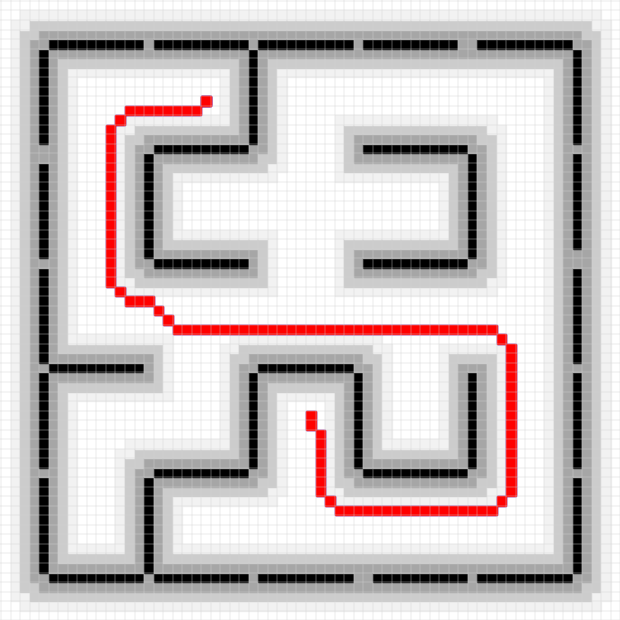
\includegraphics[width=1\linewidth]{assets/naif_2.png}
        \end{figure}
    \end{column}
    \begin{column}{.5\textwidth}
        \begin{itemize}
            \item Cet algorithme tend à longer les murs
            \item Complexité:
        \end{itemize}
        \begin{enumerate}
            \item \(O(N)\) où \(N\) est le nombre de cellules
            \item \(O(N\log(N))\)
            \item \(O(N\log(N))\)
        \end{enumerate}
        Et \(N \propto \frac{1}{p^2}\) ou \(p\) représente la précision
    \end{column}
\end{columns}
\end{frame}